\documentclass{article}

% NeurIPS 2024 style. Place neurips_2024.sty next to this file (bundled with the
% official template, also available on Overleaf). \final shows author block.
\usepackage[final]{neurips_2024}

\usepackage[utf8]{inputenc}
\usepackage[T1]{fontenc}
\usepackage{hyperref}
\usepackage{url}
\usepackage{booktabs}
\usepackage{amsfonts,amsmath}
\usepackage{graphicx}
\graphicspath{{../results/plots/}}

\title{GNN--BERT Fusion for Music Context Understanding}

\author{%
  CSE425 Project \\
  BRAC University \\
}

\begin{document}
\maketitle

\begin{abstract}
We study whether combining a graph representation of audio structure with a
pretrained language model improves music context understanding. Audio clips are
turned into \emph{segment graphs} encoded by GraphSAGE, and text (tag metadata or
free-text captions) is encoded by DistilBERT. We evaluate four tasks on
MagnaTagATune (MTAT) and MusicCaps: (1) text-only tagging, (2) graph-only
tagging, (3) graph--text fusion with ablations, and (4) contrastive
audio--caption retrieval. On MTAT top-50 tagging, both fusion variants beat
their unimodal ablations (concat Macro-F1 $0.276$, cross-attention $0.257$ vs.\
$0.224$ for either single modality), and the contrastive model reaches
Caption$\rightarrow$Audio R@10 of $23.4\%$ ($\sim$12$\times$ random) with a
zero-shot tag Macro-F1 of $0.172$. All models clearly beat a random baseline
($0.066$). Code and reproducible artifacts (seed 42) accompany the report.
\end{abstract}

\section{Introduction}
Music understanding sits between audio signal processing and natural language:
a piece has both acoustic structure (repetition, contrast, texture) and
describable semantics (genre, instrumentation, mood). Most tagging systems model
audio alone. We ask a focused question: does representing a clip's temporal
structure as a graph, and fusing it with a language model, help? We implement
the four-task pipeline from the course specification and report honest
comparisons, including ablations that isolate each modality.

\section{Method}
\paragraph{Segment graphs.}
Each clip is resampled to 22.05\,kHz mono and cut into 5\,s windows with 2.5\,s
hop. Each window (node) is a 64-dim vector: MFCC-20 and chroma-12, each summarised
by mean and standard deviation over time. Edges are (i) temporal, connecting
adjacent windows bidirectionally, and (ii) similarity, connecting non-adjacent
windows with cosine similarity $>\tau{=}0.6$ (at most 4 extra edges per node,
weighted by similarity). This captures both sequence and long-range
repetition/self-similarity.

\paragraph{Encoders.}
The graph encoder is a 2-layer GraphSAGE~\cite{hamilton2017graphsage}
(PyTorch Geometric~\cite{fey2019pyg}) with mean readout, producing a 256-dim
graph embedding $g$. Text is encoded by a fully fine-tuned
DistilBERT~\cite{sanh2019distilbert,devlin2019bert}; we use the CLS embedding
$t_{\text{CLS}}$ and the token sequence $H$.

\paragraph{Fusion (Task 3).}
The main fusion uses single-head cross-attention with the graph readout as query
and projected BERT tokens as keys/values,
$\mathrm{ctx}=\mathrm{softmax}(qK^\top/\sqrt{d})V$, and classifies from
$z=[g;\mathrm{ctx}]$ through an MLP with sigmoid outputs (BCE loss). We compare
against \texttt{concat} ($z=[g;t_{\text{CLS}}]$), \texttt{bert\_only}, and
\texttt{gnn\_only}.

\paragraph{Contrastive retrieval (Task 4).}
A dual encoder maps graphs and captions into a shared space (L2-normalised
256-dim), trained with symmetric InfoNCE~\cite{oord2018infonce,radford2021clip}
at temperature $0.07$. Branches are warm-started from the Task-1/Task-2
checkpoints. This mirrors audio--language contrastive models such as
CLAP~\cite{elizalde2023clap}.

\begin{figure}[t]
  \centering
  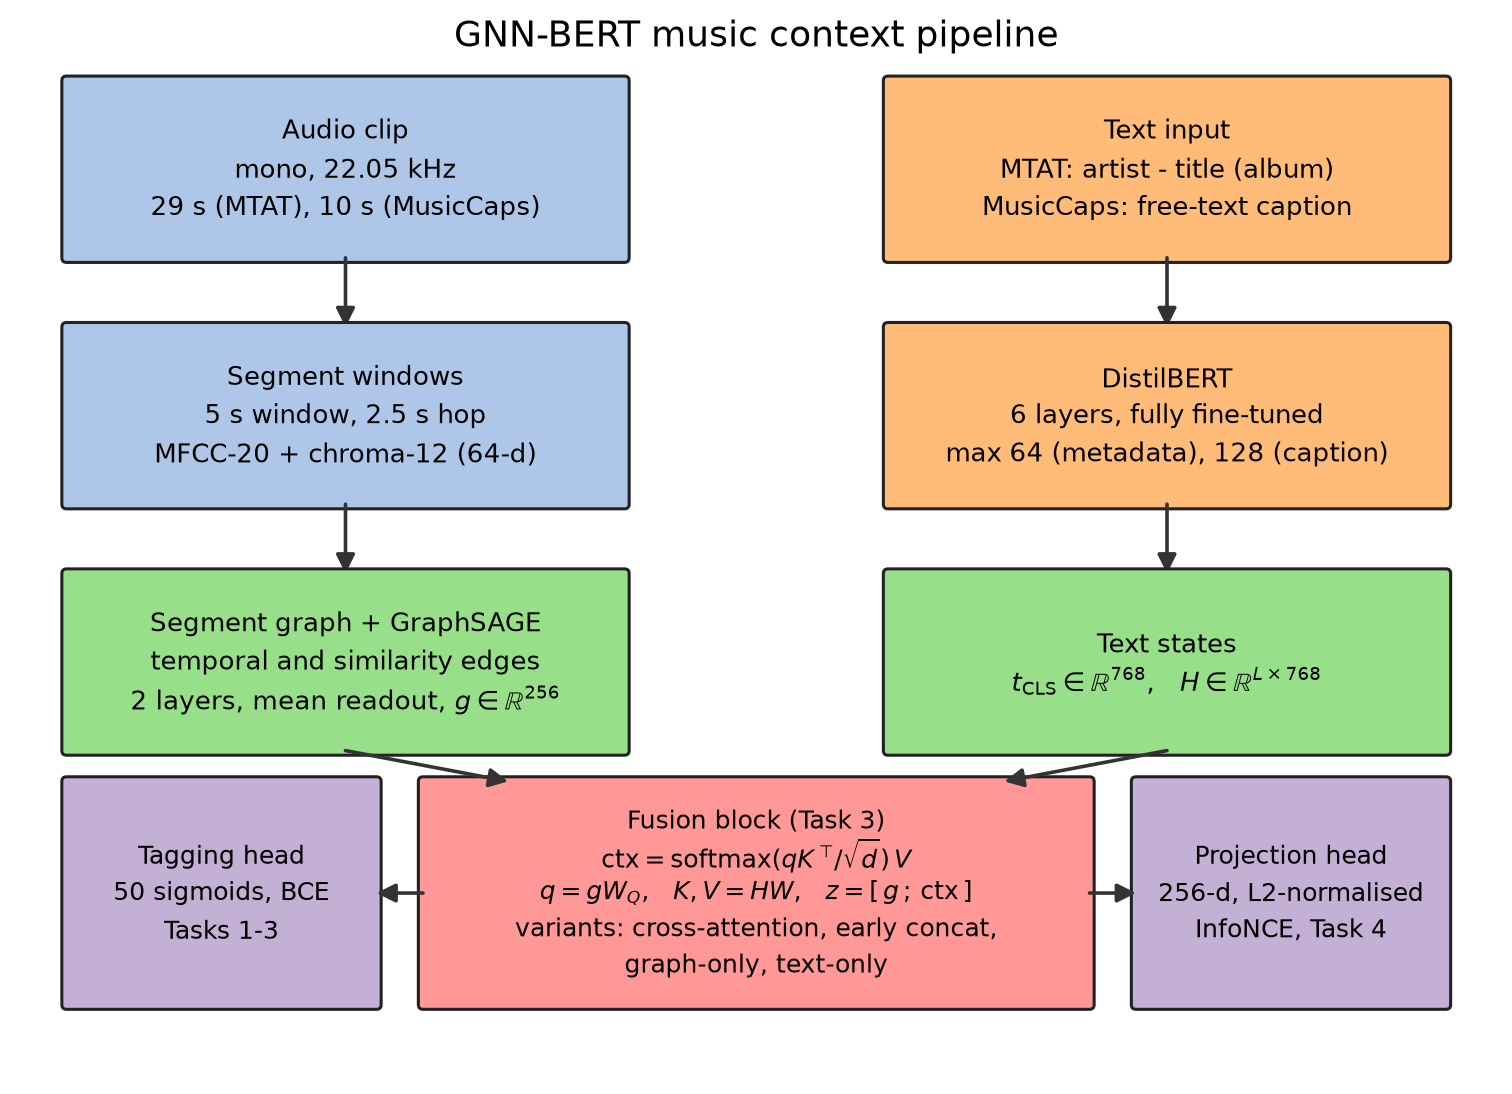
\includegraphics[width=\linewidth]{architecture.png}
  \caption{Pipeline: audio segment graph (GraphSAGE) and text (DistilBERT) are
  fused by cross-attention for tagging (Tasks 1--3) and aligned contrastively for
  retrieval (Task 4).}
  \label{fig:arch}
\end{figure}

\section{Experimental Setup}
\paragraph{Datasets.}
\textbf{MagnaTagATune}~\cite{law2009mtat} (25{,}863 clips, 29\,s) with the top-50
tags; we keep the 21{,}111 clips having at least one top-50 tag. As MTAT has no
lyrics/captions, Task-1 text is the clip metadata string
``\texttt{artist - title (album)}''. Because MTAT ships 16 folders, we use the
community folder split: train = folders \texttt{0}--\texttt{c}, val = \texttt{d},
test = \texttt{e,f} (no clip-level leakage), giving 16{,}779 / 1{,}339 / 2{,}993.
\textbf{MusicCaps}~\cite{agostinelli2023musiclm} provides 10\,s clips with
free-text captions; since YouTube blocks automated downloads, we source the audio
from the public \texttt{CLAPv2/MusicCaps} mirror (5{,}352 clips) and use a
deterministic 90/10 split (seed 42). All runs use seed 42.

\paragraph{Training.}
DistilBERT is fine-tuned at lr $2\!\times\!10^{-5}$; GNN/fusion heads at
$10^{-3}$. We use AdamW, mixed precision, and gradient accumulation to fit a 4\,GB
GPU. Task 1: 10 epochs; Task 2: 20; CNN baseline: 15; Task 3: 8 (validation
plateaus early); Task 4: 20.

\paragraph{Baselines.}
B1 random predicts each tag with its prior (analytic F1). B2 is a 4-block
CNN on log-mel spectrograms. B3 is the Task-1 BERT model.

\section{Results}
\begin{table}[t]
  \centering
  \caption{MTAT test, top-50 tags. Both fusion variants beat either unimodal
  ablation; all models beat random.}
  \label{tab:main}
  \begin{tabular}{lccc}
    \toprule
    Model & Macro-F1 & Micro-F1 & mean AUC-PR \\
    \midrule
    B1 random                 & 0.066 & 0.098 & 0.066 \\
    B3 / Task 1 BERT (metadata) & 0.195 & 0.319 & 0.300 \\
    Task 2 GraphSAGE          & 0.235 & 0.360 & 0.346 \\
    B2 CNN (log-mel)          & 0.299 & 0.432 & 0.400 \\
    \midrule
    Task 3 \texttt{bert\_only}  & 0.224 & 0.340 & 0.309 \\
    Task 3 \texttt{gnn\_only}   & 0.224 & 0.377 & 0.332 \\
    Task 3 \texttt{concat}      & \textbf{0.276} & 0.403 & 0.389 \\
    Task 3 \texttt{cross\_attn} & 0.257 & 0.382 & 0.385 \\
    \bottomrule
  \end{tabular}
\end{table}

\begin{table}[t]
  \centering
  \caption{Task 4 contrastive retrieval (MusicCaps test, 535 clips) and zero-shot
  tag transfer to MTAT. Random R@10 $\approx 1.9\%$.}
  \label{tab:retrieval}
  \begin{tabular}{lccc}
    \toprule
    Direction & R@1 & R@5 & R@10 \\
    \midrule
    Caption $\rightarrow$ Audio & 2.99 & 14.95 & 23.36 \\
    Audio $\rightarrow$ Caption & 3.74 & 13.64 & 22.06 \\
    \bottomrule
  \end{tabular}
  \quad
  \begin{tabular}{lc}
    \toprule
    Zero-shot tag probe & value \\
    \midrule
    Macro-F1 & 0.172 \\
    Micro-F1 & 0.197 \\
    mean AUC-PR & 0.185 \\
    \bottomrule
  \end{tabular}
\end{table}

\paragraph{Tagging (Tables~\ref{tab:main}).}
Audio structure alone (GraphSAGE, $0.235$) already beats sparse metadata text
(BERT, $0.195$); the raw-spectrogram CNN is strongest single model ($0.299$),
unsurprising since 64-dim segment nodes discard fine spectral detail. The key
result is the ablation: fusing modalities beats either alone --- \texttt{concat}
$0.276$ and \texttt{cross\_attn} $0.257$ vs.\ $0.224$ for both \texttt{bert\_only}
and \texttt{gnn\_only}. Simple concatenation edging out cross-attention suggests
the CLS summary already carries most of the useful text signal for these short
metadata strings.

\paragraph{Retrieval (Table~\ref{tab:retrieval}).}
On captions--audio the dual encoder reaches R@10 $\approx 23\%$, more than an
order of magnitude above chance, and transfers zero-shot to MTAT tagging
(Macro-F1 $0.172$) using only tag-name prompts, despite never seeing MTAT tags
during contrastive training.

\begin{figure}[t]
  \centering
  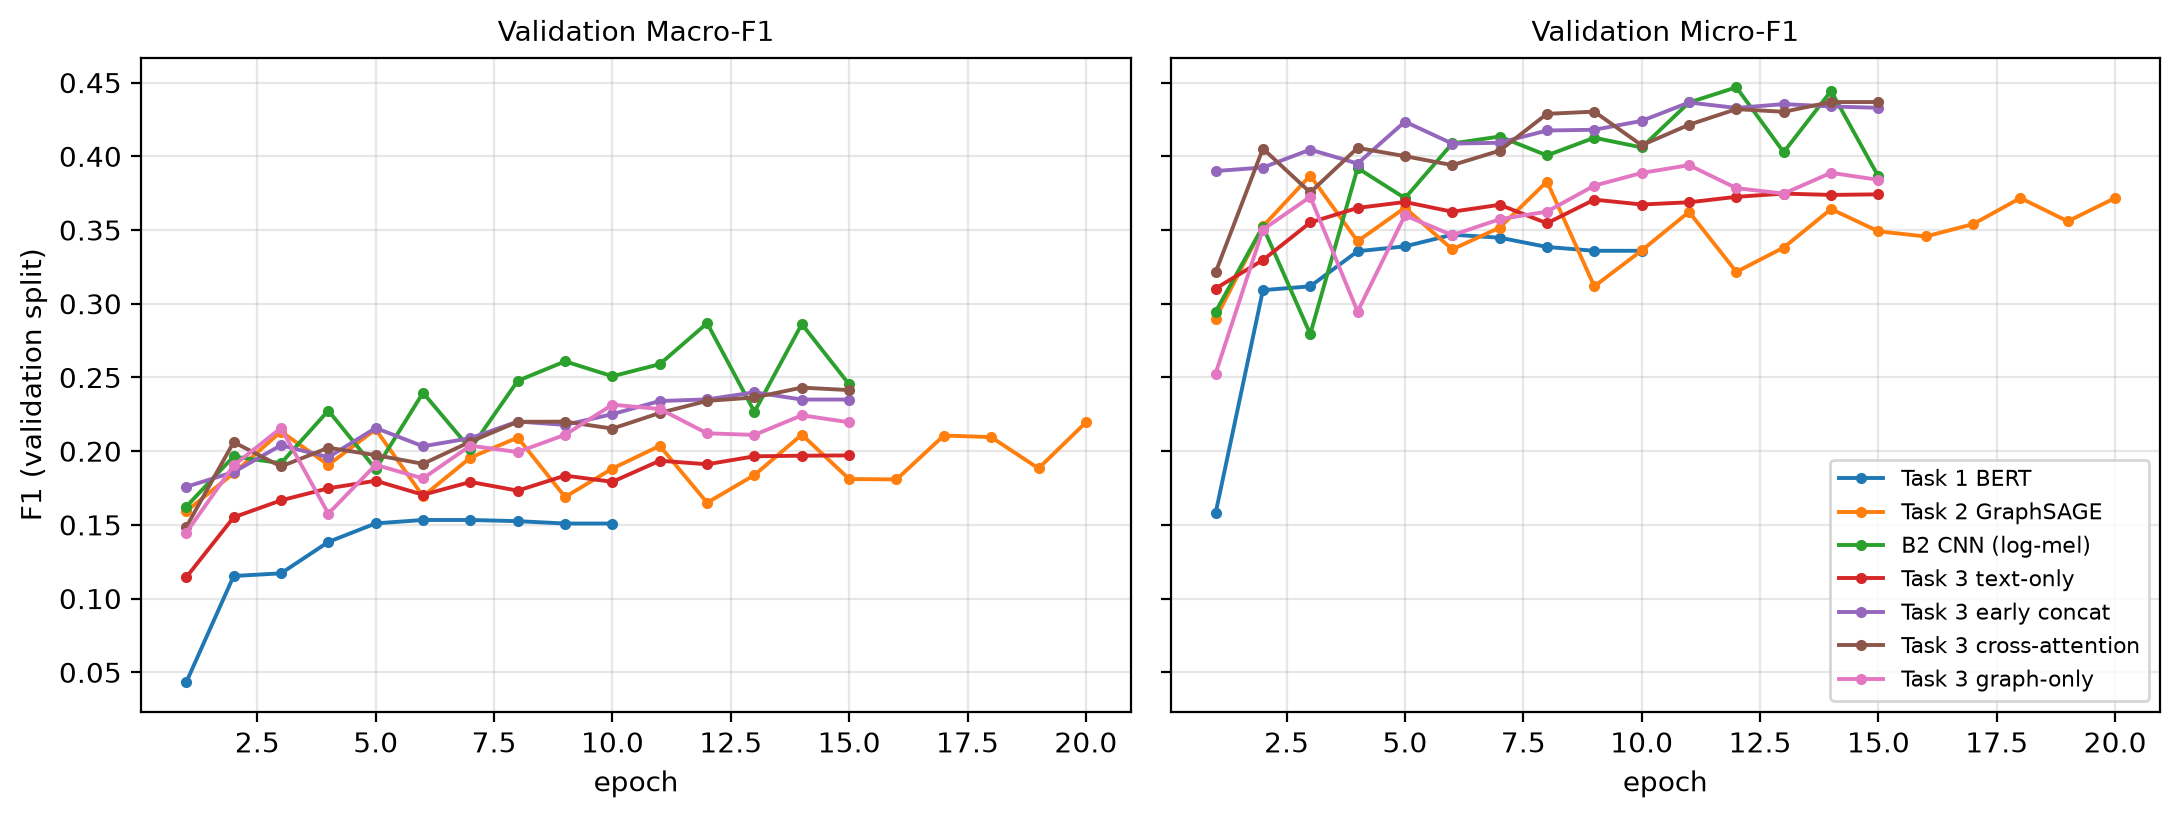
\includegraphics[width=0.9\linewidth]{f1_curves.png}
  \caption{Validation Macro-F1 vs.\ epoch across tasks/variants.}
  \label{fig:f1}
\end{figure}

\paragraph{Analysis.}
Figure~\ref{fig:tsne} shows a t-SNE of the fused Task-3 embedding on MTAT test,
coloured by dominant-tag genre umbrella: classical, electronic, world, and
acoustic clips form clearly separated regions, indicating the fusion learns
semantically organised structure. Qualitatively, the demo predicts
\{classical, opera, violin, strings\} for a Bach cantata clip (exact match), and
caption$\rightarrow$audio retrieval for a ``soft female-vocal pop'' query returns
female-vocal/pop clips. Case studies of well-retrieved clips show graphs with
several similarity edges (repeated segments), consistent with the intuition that
self-similar structure aids alignment.

\begin{figure}[t]
  \centering
  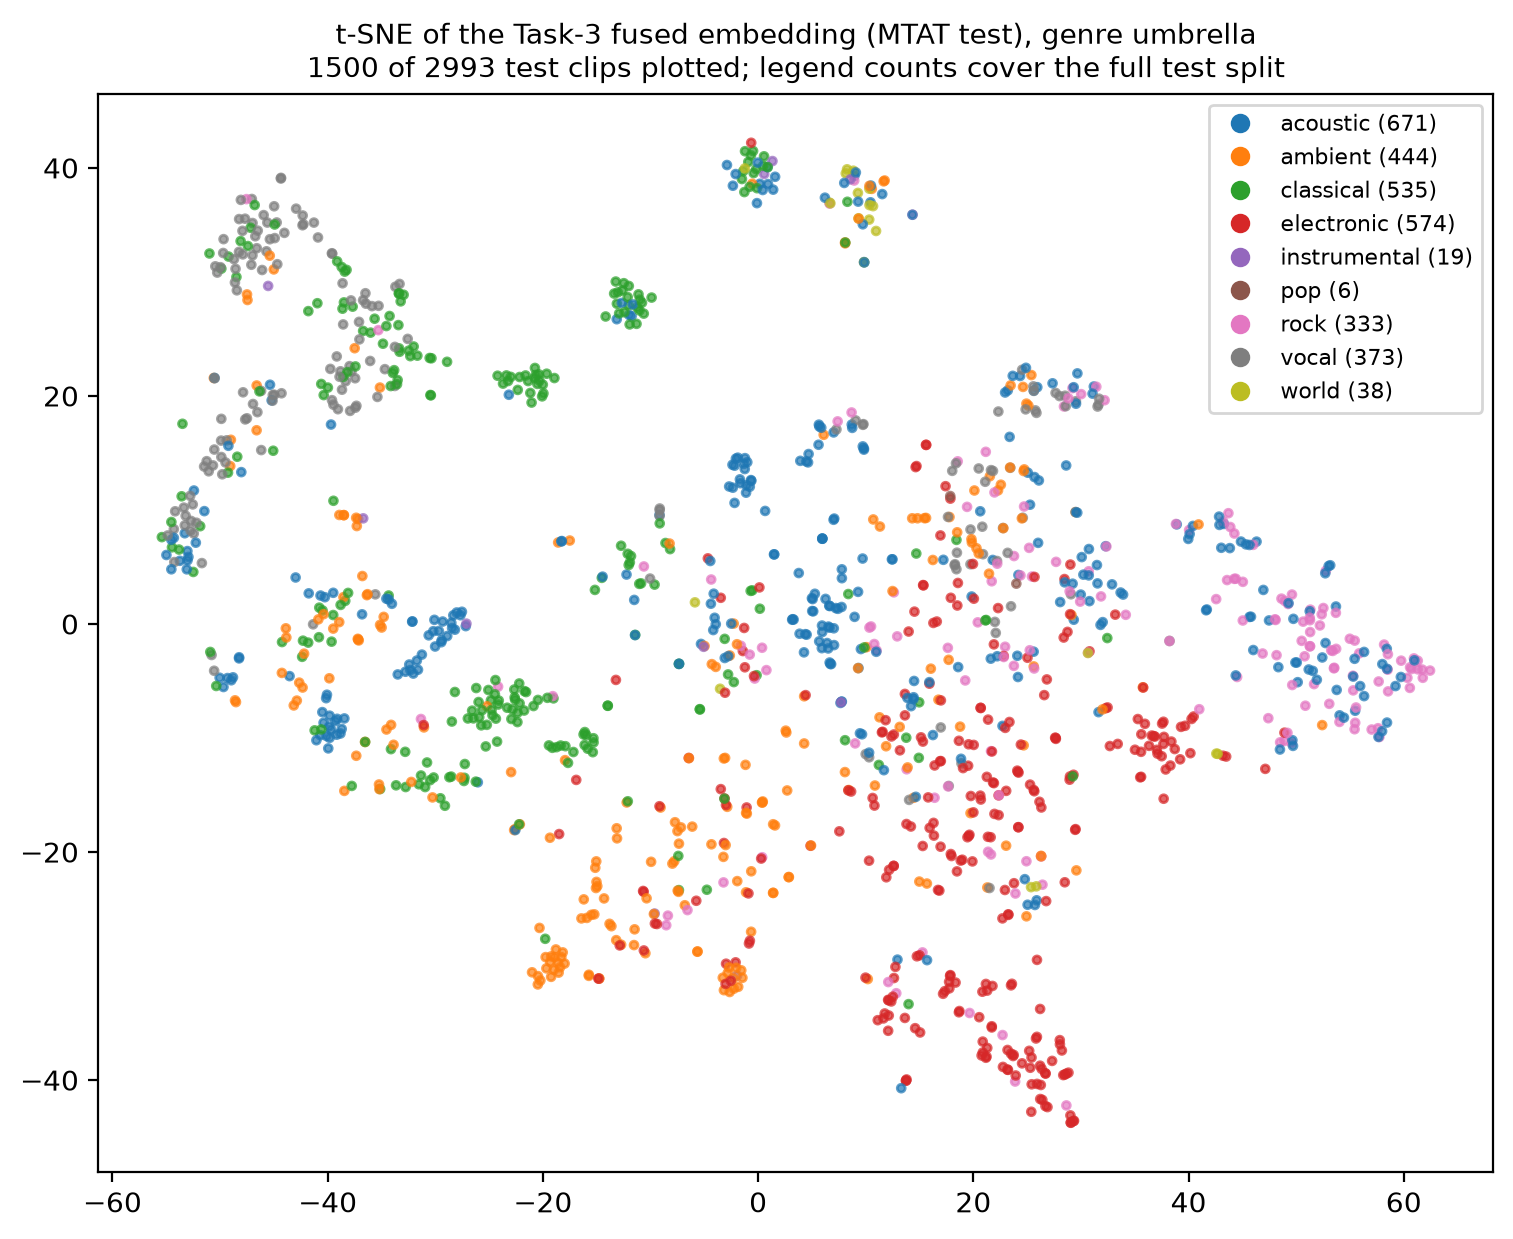
\includegraphics[width=0.75\linewidth]{tsne_task3.png}
  \caption{t-SNE of the Task-3 fused embedding $z$ (MTAT test), coloured by genre
  umbrella.}
  \label{fig:tsne}
\end{figure}

\paragraph{Limitations.}
Node features are low-dimensional hand-crafted descriptors, capping the graph
branch below the CNN; learned per-segment audio embeddings would likely close the
gap. Task-1 text is only metadata, not lyrics/captions, so the language branch is
weak on MTAT. Task 3 was trained for 8 epochs under a hardware/runtime constraint.
Human evaluation of retrieval was a single-rater self-assessment.

\section{Conclusion}
Fusing an audio segment-graph encoder with a fine-tuned language model improves
multi-label music tagging over either modality alone, and a contrastive variant
supports meaningful cross-modal retrieval and zero-shot tag transfer. The segment
graph is a lightweight, interpretable audio representation; pairing it with
stronger learned node features is a promising next step.

\bibliographystyle{plain}
\bibliography{references}

\end{document}
